\section{Zanjirning bir qismi uchun Om qonuni. Qarshilik.}


\begin{enumerate}

\item Zanjir qismidagi tok kuchi ...
\begin{enumerate}[label=\Alph*)]
\item o‘tkazgichdan o‘tgan zaryad miqdoriga teng.
\item kuchlanishga to‘g‘ri, qarshilikka teskari proporsional.
\item kuchlanish bilan qarshilik ko‘paytmasiga teng.
\item qarshilikka to‘g‘ri, kuchlanishga teskari proporsional.
\item TJY.
\end{enumerate}

\item Qarshiligi $10~\Omega$ bo‘lgan rezistordagi kuchlanish $60$ V ga teng. Undan o‘tayotgan tok kuchini toping (A).
\begin{enumerate}[label=\Alph*)]
\item $1/6$
\item 6
\item 600
\item 70
\item 50
\end{enumerate}

\item Rezistordagi kuchlanish $60$ V va undan o‘tayotgan tok kuchi $2$ A ga teng. Uning qarshiligini toping ($\Omega$).
\begin{enumerate}[label=\Alph*)]
\item $1/30$
\item 120
\item 62
\item 30
\item 58
\end{enumerate}

\item Qarshiligi $40~\Omega$ bo‘lgan rezistordan $5$ A tok o‘tmoqda. Undagi kuchlanishni toping (V).
\begin{enumerate}[label=\Alph*)]
\item $1/8$
\item 8
\item 45
\item 35
\item 200
\end{enumerate}

\item Qarshiligi $12~\Omega$ bo‘lgan rezistordagi kuchlanish $48$ V ga teng. Undan o‘tayotgan tok kuchini toping (A).
\begin{enumerate}[label=\Alph*)]
\item 4
\item $1/4$
\item 576
\item 36
\item 60
\end{enumerate}

\item Rezistordagi kuchlanish $100$ V va undan o‘tayotgan tok kuchi $5$ A ga teng. Uning qarshiligini toping ($\Omega$).
\begin{enumerate}[label=\Alph*)]
\item 500
\item $1/20$
\item 20
\item 105
\item 95
\end{enumerate}

\item Qarshiligi $25~\Omega$ bo‘lgan rezistordan $10$ A tok o‘tmoqda. Undagi kuchlanishni toping (V).
\begin{enumerate}[label=\Alph*)]
\item 15
\item 0,4
\item 2,5
\item 250
\item 35
\end{enumerate}

\item Qarshiligi $34~\Omega$ bo‘lgan o‘tkazgich orqali $2$ A tok o‘tkazish uchun o‘tkazgich uchlariga qanday kuchlanish (V) qo‘yish kerak?
\begin{enumerate}[label=\Alph*)]
\item 34
\item 17
\item 68
\item 51
\item 10
\end{enumerate}

\item Agar rezistorning qarshiligi $R=6~\Omega$ va undan o‘tayotgan tok kuchi $I=2$ A bo‘lsa, B va A nuqtadagi potensiallar farqi $\varphi_B-\varphi_A$ ni (V) toping.

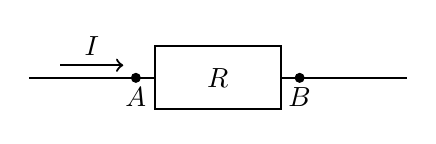
\begin{tikzpicture}[scale=0.8]

\draw[thick] (0,0) -- (2,0);
\draw[thick,->] (0.5,0.2) -- (1.5,0.2) node at (1,0.5) {$I$};
\node at (3,0) {$R$};
\filldraw (1.7,0) circle (2pt) node[below] (1.7,0) {$A$};
\filldraw (4.3,0) circle (2pt) node[below] (4.3,0) {$B$};

\draw[thick] (2,-0.5) rectangle (4,0.5);
\draw[thick] (4,0) -- (6,0);

\end{tikzpicture}



\begin{enumerate}[label=\Alph*)]
\item $-12$
\item 8
\item $-8$
\item 12
\item 3
\end{enumerate}

\item Uchlaridagi kuchlanish $24$ V, qarshiligi $20~\Omega$ bo‘lgan o‘tkazgichdan $60$ s vaqt ichida qancha (C) zaryad o‘tadi?
\begin{enumerate}[label=\Alph*)]
\item 17
\item 40
\item 24
\item 72
\item 25
\end{enumerate}

\item Quyida qarshiligi $12~\Omega$ bo‘lgan o‘tkazgichning uchlariga qo‘yilgan potensiallar farqining vaqtga bog‘liqligi ko‘rsatilgan. O‘tkazgichdan o‘tgan tok kuchini (A) aniqlang.

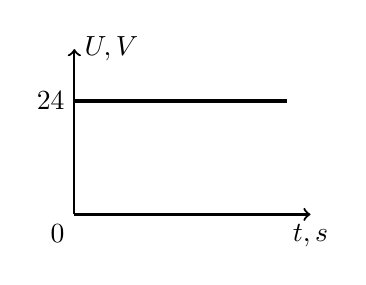
\begin{tikzpicture}[scale=0.6]
    % Koordinata o'qlari
    \draw[->, thick] (0,0) -- (5,0) node[below] { $t, s$}; % Vaqt o'qi
    \draw[->, thick] (0,0) -- (0,3.5) node[right] { $U, V$}; % Kuchlanish o'qi

    % Grafik chizig'i (O'zgarmas kuchlanish 24 V)
    % Masshtabni moslash uchun 2.4 birlik balandlikda chizamiz
    \draw[very thick] (0,2.4) -- (4.5,2.4);

    % Qiymatlarni belgilash
    \node[left] at (0,2.4) { $24$}; % Kuchlanish qiymati
    \node[below left] at (0,0) { $0$}; % Koordinata boshi

\end{tikzpicture}

\begin{enumerate}[label=\Alph*)]
\item 0
\item 0,5
\item 2
\item 1
\item 4
\end{enumerate}

\item Qarshiligi $12~\Omega$ bo‘lgan o‘tkazgichdan $3$ minutda $90$ C elektr miqdori o‘tgan. Bu o‘tkazgich uchlaridagi kuchlanishni toping (V).
\begin{enumerate}[label=\Alph*)]
\item 12
\item 6
\item 10
\item 9
\item 15
\end{enumerate}

\item Qarshiligi $2~\Omega$ bo‘lgan silindrsimon metall o‘tkazgich uchlariga $24$ V kuchlanish qo‘yilgan. Bu o‘tkazgich ko‘ndalang kesimidan $32$ s da nechta elektron o‘tadi?
\begin{enumerate}[label=\Alph*)]
\item $2,4\cdot10^{21}$
\item $2,4\cdot10^{20}$
\item $2,4\cdot10^{22}$
\item $2,4\cdot10^{19}$
\end{enumerate}

\item O‘zgarmas kuchlanish manbaiga ulangan reostatning surqichi surilib, qarshiligi $4$ marta kamaytirilsa, undagi tok kuchi qanday o‘zgaradi?
\begin{enumerate}[label=\Alph*)]
\item 2 marta ortadi.
\item 2 marta kamayadi.
\item 4 marta ortadi.
\item o‘zgarmaydi.
\item 4 marta kamayadi.
\end{enumerate}

\item Reostatdagi kuchlanish $2$ marta orttirildi, uning qarshiligi esa $3$ marta kamaytirildi. Reostatdagi tok qanday o‘zgaridi?
\begin{enumerate}[label=\Alph*)]
\item 1,5 marta kamaydi.
\item 1,5 marta ortdi.
\item o‘zgarmadi.
\item 6 marta kamaydi.
\item 6 marta ortdi.
\end{enumerate}

\item Elektr zanjirining o‘zgarmas qarshilikka ega bo‘lgan qismidan o‘tayotgan tok kuchi $4$ marta oshirilsa, shu qismdagi kuchlanish qanday o‘zgaradi?
\begin{enumerate}[label=\Alph*)]
\item 4 marta kamayadi.
\item 4 marta oshadi.
\item 2 marta kamayadi.
\item 2 marta oshadi.
\item o‘zgarmaydi.
\end{enumerate}

\item O‘tkazgich uchlaridagi kuchlanish ...
\begin{enumerate}[label=\Alph*)]
\item o‘tkazgichdan o‘tayotgan tok kuchi bilan o‘tkazgich qarshiligi ko‘paytmasiga teng.
\item o‘tkazgich ichida zaryadni ko‘chirishda bajarilgan ishga teng.
\item o‘tkazgich qarshiligini tok kuchiga nisbatiga teng.
\item o‘tkazgichdan o‘tayotgan tok kuchining o‘tkazgich qarshiligiga nisbatiga teng.
\item TJY.
\end{enumerate}

\item C/s birlik javobda keltirilgan birliklarning qaysi biriga teng kuchli?
\begin{enumerate}[label=\Alph*)]
\item V/$\Omega$
\item V/m
\item V
\item V$\cdot$m
\item V$\cdot\Omega$
\end{enumerate}

\item Quyidagilardan qaysi biri Xalqaro Birliklar Sistemasi (SI) dagi asosiy birlik hisoblanadi?
\begin{enumerate}[label=\Alph*)]
\item Volt
\item Kulon
\item Amper
\item Om
\item Farad
\end{enumerate}

\item Quyida keltirilgan birliklarning qaysilari kuchlanishning birligi bo‘la olmaydi?\\
1) A/s; \quad
2) J/C;\quad
3) A$\cdot$s$\Omega$;\quad
4) N/C;\quad
5) Nm/C;\quad
6) W/A;\quad
7) V.

\begin{enumerate}[label=\Alph*)]
\item 1, 2, 4
\item 1, 4
\item 1, 2, 3, 4, 5, 6
\item 1, 4, 6
\item 2, 3, 5, 6
\end{enumerate}

\item O‘lchamligi V$^2\cdot$s/J ko‘rinishida bo‘lgan fizik kattalikni ayting.
\begin{enumerate}[label=\Alph*)]
\item kuchlanish.
\item solishtirma qarshilik.
\item qarshilik.
\item zichlik.
\item tok kuchi.
\end{enumerate}

\item Rasmda to‘rtta har xil o‘tkazgichdagi tok kuchining kuchlanishga bog‘lanish grafiglari berilgan. O‘tkazgichlar qarshiliklari haqida nima deyish mumkin?

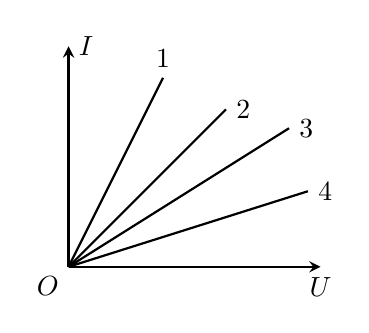
\begin{tikzpicture}[>=stealth, scale=0.8]
    % Koordinata o'qlari
    \draw[->, thick] (0,0) -- (4,0) node[below] {$U$}; % Kuchlanish o'qi
    \draw[->, thick] (0,0) -- (0,3.5) node[right] {$I$}; % Tok kuchi o'qi
    \node[below left] at (0,0) {$O$};

    % To'rtta o'tkazgichning grafik chiziqlari
    \draw[thick] (0,0) -- (1.5, 3) node[above] {1};
    \draw[thick] (0,0) -- (2.5, 2.5) node[right] {2};
    \draw[thick] (0,0) -- (3.5, 2.2) node[right] {3};
    \draw[thick] (0,0) -- (3.8, 1.2) node[right] {4};

\end{tikzpicture}

\begin{enumerate}[label=\Alph*)]
\item $R_1$ eng katta, $R_4$ eng kichik.
\item $R_4$ eng katta, $R_1$ eng kichik.
\item $R_1=R_2=R_3=R_4$.
\item $R_2>R_1>R_3>R_4$.
\item $R_1+R_2=R_3+R_4$.
\end{enumerate}

\item Rasmda uchta turli o‘tkazgich uchun tok kuchining kuchlanishga bog‘lanish grafiglari berilgan. Grafiklardan foydalanib, qaysi o‘tkazgichning qarshiligi eng katta ekanligini aniqlang.

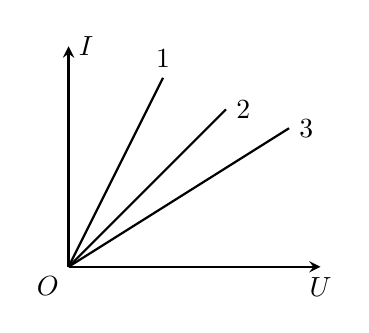
\begin{tikzpicture}[>=stealth, scale=0.8]
    % Koordinata o'qlari
    \draw[->, thick] (0,0) -- (4,0) node[below] {$U$}; % Kuchlanish o'qi
    \draw[->, thick] (0,0) -- (0,3.5) node[right] {$I$}; % Tok kuchi o'qi
    \node[below left] at (0,0) {$O$};

    % To'rtta o'tkazgichning grafik chiziqlari
    \draw[thick] (0,0) -- (1.5, 3) node[above] {1};
    \draw[thick] (0,0) -- (2.5, 2.5) node[right] {2};
    \draw[thick] (0,0) -- (3.5, 2.2) node[right] {3};
    

\end{tikzpicture}

\begin{enumerate}[label=\Alph*)]
\item 1
\item 2
\item 3
\item uchala o‘tkazgich qarshiligi bir xil.
\item TJY.
\end{enumerate}

\item O‘tkazgichdan o‘tayotgan tok kuchining kuchlanishga bog‘lanish grafigidan foydalanib, o‘tkazgichning qarshiligini hisoblang ($\Omega$).

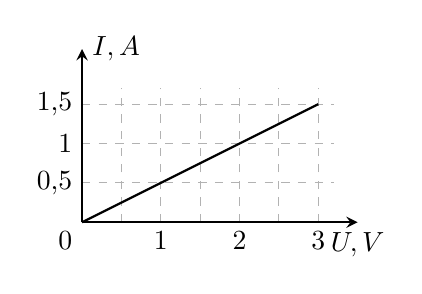
\begin{tikzpicture}[>=stealth, scale=1]
    % Punktir to'r (grid) chizish
    \draw[dashed, thin, gray!60, step=0.5] (0,0) grid (3.2, 1.7);

    % Koordinata o'qlari
    \draw[->, thick] (0,0) -- (3.5,0) node[below] {$U, \text{V}$}; % Kuchlanish o'qi
    \draw[->, thick] (0,0) -- (0,2.2) node[right] {$I, \text{A}$};   % Tok kuchi o'qi
    \node[below left] at (0,0) {0};

    % Grafik chizig'i (I = 0.5 * U bog'liqligi)
    % U=1 da I=0.5; U=2 da I=1; U=3 da I=1.5
    \draw[thick] (0,0) -- (3, 1.5); 

    % Gorizontal o'qdagi (U) qiymatlar
    \node[below] at (1,0) {1};
    \node[below] at (2,0) {2};
    \node[below] at (3,0) {3};

    % Vertikal o'qdagi (I) qiymatlar
    \node[left] at (0,0.5) {0,5};
    \node[left] at (0,1) {1};
    \node[left] at (0,1.5) {1,5};

\end{tikzpicture}

\begin{enumerate}[label=\Alph*)]
\item 0,5
\item 1
\item 1,5
\item 2
\item 4,5
\end{enumerate}

\item Grafikdan foydalanib, o‘tkazgichning qarshiligini toping ($\Omega$).

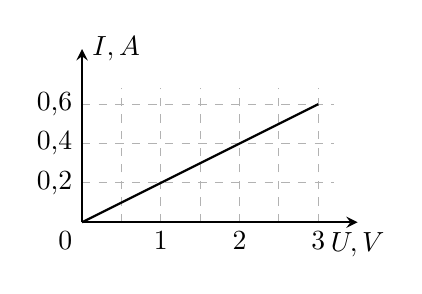
\begin{tikzpicture}[>=stealth, scale=1]
    % Punktir to'r (grid) chizish
    \draw[dashed, thin, gray!60, step=0.5] (0,0) grid (3.2, 1.7);

    % Koordinata o'qlari
    \draw[->, thick] (0,0) -- (3.5,0) node[below] {$U, \text{V}$}; % Kuchlanish o'qi
    \draw[->, thick] (0,0) -- (0,2.2) node[right] {$I, \text{A}$};   % Tok kuchi o'qi
    \node[below left] at (0,0) {0};

    % Grafik chizig'i (I = 0.5 * U bog'liqligi)
    % U=1 da I=0.5; U=2 da I=1; U=3 da I=1.5
    \draw[thick] (0,0) -- (3, 1.5); 

    % Gorizontal o'qdagi (U) qiymatlar
    \node[below] at (1,0) {1};
    \node[below] at (2,0) {2};
    \node[below] at (3,0) {3};

    % Vertikal o'qdagi (I) qiymatlar
    \node[left] at (0,0.5) {0,2};
    \node[left] at (0,1) {0,4};
    \node[left] at (0,1.5) {0,6};

\end{tikzpicture}

\begin{enumerate}[label=\Alph*)]
\item 0,2
\item 1,8
\item 5
\item 0,8
\item 3,6
\end{enumerate}

\item O‘tkazgichlarning volt–amper xarakteristikasidan foydalanib, 1-o‘tkazgich qarshiligining 2-o‘tkazgich qarshiligiga nisbatini toping.


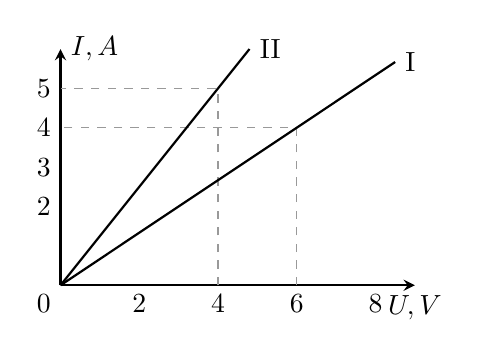
\begin{tikzpicture}[>=stealth, scale=0.5]
    % Koordinata o'qlari
    \draw[->, thick] (0,0) -- (9,0) node[below] {$U, \text{V}$}; % Kuchlanish o'qi
    \draw[->, thick] (0,0) -- (0,6) node[right] {$I, \text{A}$}; % Tok kuchi o'qi
    \node[below left] at (0,0) {0};

    % Nuqtalarni ko'rsatuvchi punktir chiziqlar
    \draw[dashed, gray!80] (4,0) -- (4,5) -- (0,5); % II-chiziq uchun nuqta (4; 5)
    \draw[dashed, gray!80] (6,0) -- (6,4) -- (0,4); % I-chiziq uchun nuqta (6; 4)

    % Grafik chiziqlari
    \draw[thick] (0,0) -- (4.8, 6) node[right] {II}; % II-o'tkazgich grafigi
    \draw[thick] (0,0) -- (8.5, 5.67) node[right] {I}; % I-o'tkazgich grafigi

    % Qiymatlarni belgilash (U o'qi)
    \node[below] at (2,0) {2};
    \node[below] at (4,0) {4};
    \node[below] at (6,0) {6};
    \node[below] at (8,0) {8};

    % Qiymatlarni belgilash (I o'qi)
    \node[left] at (0,2) {2};
    \node[left] at (0,3) {3};
    \node[left] at (0,4) {4};
    \node[left] at (0,5) {5};

\end{tikzpicture}

\begin{enumerate}[label=\Alph*)]
\item 2
\item 1,95
\item 1,78
\item 1,1
\item 1,875
\end{enumerate}

\item Chizmadan foydalanib, qarshilik $2,5~\Omega$ va $1~\Omega$ bo‘lgandagi toklarning nisbatini toping.

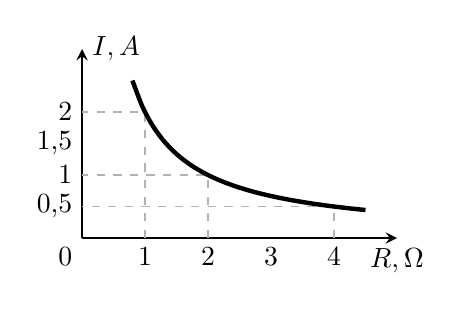
\begin{tikzpicture}[>=stealth, scale=0.8]
    % Koordinata o'qlari
    \draw[->, thick] (0,0) -- (5,0) node[below] {$R, \Omega$}; % Qarshilik o'qi
    \draw[->, thick] (0,0) -- (0,3) node[right] {$I, \text{A}$}; % Tok kuchi o'qi
    \node[below left] at (0,0) {0};

    % Nuqtalarni belgilash uchun punktir chiziqlar (Setka)
    \draw[dashed, gray!60] (1,0) -- (1,2) -- (0,2);
    \draw[dashed, gray!60] (2,0) -- (2,1) -- (0,1);
    \draw[dashed, gray!60] (4,0) -- (4,0.5) -- (0,0.5);

    % Grafik chizig'i (I = 2/R bog'liqligi)
    \draw[ultra thick, domain=0.8:4.5, smooth] plot (\x, {2/\x});

    % Qiymatlarni belgilash (R o'qi)
    \node[below] at (1,0) {1};
    \node[below] at (2,0) {2};
    \node[below] at (3,0) {3};
    \node[below] at (4,0) {4};

    % Qiymatlarni belgilash (I o'qi)
    \node[left] at (0,0.5) {0,5};
    \node[left] at (0,1) {1};
    \node[left] at (0,1.5) {1,5};
    \node[left] at (0,2) {2};

\end{tikzpicture}

\begin{enumerate}[label=\Alph*)]
\item 2,5
\item 0,3
\item 2
\item 0,4
\item 0,1
\end{enumerate}

\item O‘tkazgichning qarshiligi nimaga bog‘liq?
\begin{enumerate}[label=\Alph*)]
\item tok kuchiga.
\item kuchlanishga.
\item o‘tkazgich materiali va geometrik o‘lchamlariga.
\item tok zichligiga.
\item o‘tkazgichdagi tok kuchi va kuchlanishga.
\end{enumerate}

\item O‘tkazgich uchlaridagi kuchlanishni orttirsak, uning qarshiligi...
\begin{enumerate}[label=\Alph*)]
\item ortadi.
\item o‘zgarmaydi.
\item kamayadi.
\item ortishi ham, kamayishi ham mumkin.
\item TJY.
\end{enumerate}

\item Berilgan formulalardan qaysi biri o‘tkazgich qarshiligining uning uzunligiga bog‘lanishini ifodalaydi?
\begin{enumerate}[label=\Alph*)]
\item $R=R_0(1+\alpha t)$.
\item $R=\dfrac{U}{I}$.
\item $R=\rho\dfrac{l}{S}$.
\item $R=\dfrac{Q}{I^2t}$.
\item $R=\dfrac{P}{I^2}$.
\end{enumerate}

\item Cho‘g‘lanma lampaning spiralini yasash uchun uzunligi $40$ cm va ko‘ndalang kesim yuzi $0,002$ mm$^2$ bo‘lgan volfram sim olingan. Volframning solishtirma qarshiligi $5,5\cdot10^{-8}~\Omega\cdot$m. Spiralning qarshiligini toping ($\Omega$)?
\begin{enumerate}[label=\Alph*)]
\item 0,11
\item 1,1
\item 5,5
\item 11
\item 110
\end{enumerate}

\item Uzunligi $50$ m va ko‘ndalang kesim yuzi $34$ mm$^2$ bo‘lgan mis simning qarshiligini toping (m$\Omega$). Misning solishtirma qarshiligi $1,7\cdot10^{-8}~\Omega\cdot$m.
\begin{enumerate}[label=\Alph*)]
\item 25
\item 5
\item 50
\item 500
\item 5000
\end{enumerate}

\item Uzunligi $210$ m bo‘lgan nikelin simning qarshiligi $14,7~\Omega$ ga teng. Uning ko‘ndalang kesim yuzini toping (mm$^2$). $\rho=4,2\cdot10^{-7}~\Omega\cdot$m.
\begin{enumerate}[label=\Alph*)]
\item 1
\item 4
\item 1,5
\item 6
\item 4,5
\end{enumerate}

\item Ko‘ndalang kesim yuzi $0,5$ cm$^2$ bo‘lgan aluminiy simning qarshiligi $2,8~\Omega$ bo‘lsa. Simning uzunligini toping (m). $\rho=2,8\cdot10^{-8}~\Omega\cdot$m.
\begin{enumerate}[label=\Alph*)]
\item 1,4
\item 5
\item 50
\item 500
\item 5000
\end{enumerate}

\item Ko‘ndalang kesim yuzi $0,17$ mm$^2$ bo‘lgan mis simning qarshiligi $9~\Omega$ bo‘lishi uchun uzunligi necha metr bo‘lishi kerak? Misning solishtirma qarshiligi $1,7\cdot10^{-8}~\Omega\cdot$m.
\begin{enumerate}[label=\Alph*)]
\item 900
\item 90
\item 170
\item 200
\item 270
\end{enumerate}

\item Quyida keltirilgan mis simlarning qaysi biri eng katta qarshilikka ega?

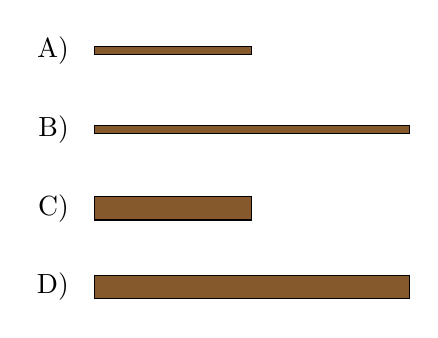
\begin{tikzpicture}
    % Sim A (O'rtacha uzunlik, ingichka)
    \node[left] at (-0.2, 3) {A)};
    \draw[fill=brown!70!black] (0, 2.95) rectangle (2, 3.05);

    % Sim B (Uzun, ingichka)
    \node[left] at (-0.2, 2) {B)};
    \draw[fill=brown!70!black] (0, 1.95) rectangle (4, 2.05);

    % Sim C (O'rtacha uzunlik, yo'g'on)
    \node[left] at (-0.2, 1) {C)};
    \draw[fill=brown!70!black] (0, 0.85) rectangle (2, 1.15);

    % Sim D (Uzun, yo'g'on)
    \node[left] at (-0.2, 0) {D)};
    \draw[fill=brown!70!black] (0, -0.15) rectangle (4, 0.15);
\end{tikzpicture}


\item $12$ mV kuchlanish ulangan uzunligi $10$ m va kesimi $2$ mm$^2$ bo‘lgan po‘lat simdagi tok kuchini aniqlang (mA). $\rho=12\cdot10^{-8}~\Omega\cdot$m.
\begin{enumerate}[label=\Alph*)]
\item 20
\item 17
\item 10
\item 0,2
\item 0,1
\end{enumerate}

\item Ko‘ndalang kesimi $150$ mm$^2$, solishtirma qarshiligi $2,8\cdot10^{-8}~\Omega\cdot$m bo‘lgan $150$ km uzunlikdagi simdan o‘zgarmas elektr toki uzatish liniyasi tortilgan. Agar tok kuchi $100$ A bo‘lsa, liniyadagi kuchlanish tushuvi necha Volt bo‘ladi?
\begin{enumerate}[label=\Alph*)]
\item 280
\item 5600
\item 2800
\item 560
\item 1400
\end{enumerate}

\item Uzunligi $500$ km, ko‘ndalang kesimi yuzi $10$ mm$^2$ bo‘lgan alyuminiy simdan $10$ mA tok o‘tayotgan bo‘lsa, uning uchlaridagi kuchlanish necha Volt? Alyuminiyning solishtirma qarshiligi $2,8\cdot10^{-8}~\Omega\cdot$m.
\begin{enumerate}[label=\Alph*)]
\item 56
\item 50
\item 35
\item 28
\item 14
\end{enumerate}

\item Ko‘ndalang kesimi $1$ mm$^2$ bo‘lgan nikelin simdan yasalgan reostatga ulangan ampermetr $20$ A ni, voltmetr esa $210$ V ni ko‘rsatadi ($\rho=4,2\cdot10^{-7}~\Omega\cdot$m). Reostat simining uzunligi necha metr?
\begin{enumerate}[label=\Alph*)]
\item 150
\item 180
\item 200
\item 250
\item 300
\end{enumerate}

\item O‘tkazgichning kesim yuzi $2$ marta, uzunligi esa $3$ marta oshsa, uning qarshiligi qanday o‘zgaradi?
\begin{enumerate}[label=\Alph*)]
\item 3 marta kamayadi.
\item 1,5 marta ortadi.
\item 3 marta ortadi.
\item 1,5 marta kamayadi.
\item o‘zgarmaydi.
\end{enumerate}

\item Mis simning qarshiligi $6~\Omega$. Shu simdan ko‘ndalang kesimi yuzi $3$ marta, uzunligi esa $2$ marta katta bo‘lgan mis simning qarshiligi qanday ($\Omega$)?
\begin{enumerate}[label=\Alph*)]
\item 3
\item 4
\item 8
\item 9
\item 10
\end{enumerate}

\item Mis simning elektr qarshiligi $6~\Omega$ ga teng. Uzunligi $3$ marta, diametri $2$ marta katta bo‘lgan mis simning qarshiligi qanday ($\Omega$)?
\begin{enumerate}[label=\Alph*)]
\item 72
\item 9
\item 8
\item 4
\item 4,5
\end{enumerate}

\item Mis simning elektr qarshiligi $6~\Omega$ ga teng. Uzunligi $3$ marta, diametri $2$ marta kichik bo‘lgan mis simning qarshiligi qanday ($\Omega$)?
\begin{enumerate}[label=\Alph*)]
\item 72
\item 9
\item 8
\item 4,5
\item 4
\end{enumerate}

\item Uzunligi $l$, ko‘ndalang kesim yuzi $S$ bo‘lgan o‘tkazgich $4~\Omega$ elektr qarshilikka ega. Xuddi moddadan yasalgan, uzunligi $2l$, ko‘ndalang kesimi $S/4$ bo‘lgan o‘tkazgich necha qarshilikka ega bo‘ladi?
\begin{enumerate}[label=\Alph*)]
\item 32
\item 16
\item 8
\item 24
\item 4
\end{enumerate}

\item Birinchi o‘tkazgichning uzunligi $1$ m, ko‘ndalang kesim yuzi $1$ mm$^2$, ikkinchi o‘tkazgichning uzunligi $2$ m, ko‘ndalang kesim yuzi $0,5$ mm$^2$. Bu o‘tkazgichlarning qarshiliklari $R_1$ va $R_2$ qanday munosabatda bo‘ladi?
\begin{enumerate}[label=\Alph*)]
\item $R_1=R_2$.
\item $R_1=4R_2$
\item aniqlab bo‘lmaydi.
\item $R_2=2R_1$
\item $R_2=4R_1$
\end{enumerate}

\item Alyuminiydan yasalgan bir xil uzunlikdagi ikki simdan birining qarshiligi $2,7~\Omega$, ikkinchisiniki $1,8~\Omega$. Birinchi simning ko‘ndalang kesim yuzi $4$ mm$^2$. Ikkinchi simning ko‘ndalang kesim yuzi qanday (mm$^2$)?
\begin{enumerate}[label=\Alph*)]
\item 9
\item 18
\item 12
\item 6
\item 3
\end{enumerate}

\item Uzunliklari bir xil, ko‘ndalang kesimlari $S_1=2S_2$ va solishtirma qarshiliklari $\rho_2=2\rho_1$ bo‘lgan ikkita o‘tkazgich qarshiliklarining nisbati $R_2/R_1$ ni aniqlang.
\begin{enumerate}[label=\Alph*)]
\item 0,25
\item 0,5
\item 2
\item 4
\item 8
\end{enumerate}

\item Uzunligi $1$ m va ko‘ndalang kesim yuzi $0,5$ mm$^2$ bo‘lgan o‘tkazgichning qarshiligi teng qarshilik hosil qilish uchun, o‘sha materialdan yasalgan va ko‘ndalang kesim yuzi $10$ mm$^2$ bo‘lgan simdan necha metr olish kerak?
\begin{enumerate}[label=\Alph*)]
\item 10
\item 20
\item 30
\item 40
\item 50
\end{enumerate}

\item Ko‘ndalang kesim yuzi $1$ mm$^2$ va og‘irligi $105$ N bo‘lgan kumush simning qarshiligini toping ($\Omega$)? Kumushning zichligi $10500$ kg/m$^3$, solishtirma qarshiligi $1,6\cdot10^{-8}~\Omega\cdot$m.
\begin{enumerate}[label=\Alph*)]
\item 16
\item 8
\item 32
\item 40
\item 48
\end{enumerate}

\item Agar o‘tkazgich uchlaridagi kuchlanish $2$ marta kamaytirilsa va uning uzunligi $2$ marta orttirilsa, undan o‘tayotgan tok kuchi qanday o‘zgaradi?
\begin{enumerate}[label=\Alph*)]
\item o‘zgarmaydi.
\item 4 marta kamayadi.
\item 4 marta ortadi.
\item 2 marta ortadi.
\item 2 marta ortadi.
\end{enumerate}

\item Bir simning uzunligi $20$ cm, ikkinchisiniki $1,6$ m. Simlarning ko‘ndalang kesimi va materiallari bir xil. Qaysi simning qarshiligi katta va necha marta katta?
\begin{enumerate}[label=\Alph*)]
\item birinchisiniki, 3,2 marta.
\item ikkinchisiniki, 3,2 marta.
\item bir xil.
\item birinchisiniki, 8 marta.
\item ikkinchisiniki, 8 marta.
\end{enumerate}

\item Agar metall simning uzunligi va radiusi $4$ marta orttirilsa, uning qarshiligi qanday o‘zgaradi?
\begin{enumerate}[label=\Alph*)]
\item 4 marta kamayadi.
\item 2 marta ortadi.
\item o‘zgarmaydi.
\item 2 marta kamayadi.
\item 4 marta ortadi.
\end{enumerate}

\item Simni cho‘zib, $3$ marta uzaytirilsa, qarshiligi necha marta ortadi?
\begin{enumerate}[label=\Alph*)]
\item 9
\item 4
\item 2
\item 3
\item o‘zgarmaydi.
\end{enumerate}

\item Manbaning kuchlanishi $2$ marta orttirilsa, rezistor qarshiligi qanday o‘zgaridi?
\begin{enumerate}[label=\Alph*)]
\item 2 marta ortadi.
\item 2 marta kamayadi.
\item 4 marta ortadi.
\item o‘zgarmaydi.
\item 4 marta kamayadi.
\end{enumerate}

\item Zanjirdagi tok kuchi $5$ marta orttirilsa, rezistorning qarshiligi qanday o‘zgaradi?
\begin{enumerate}[label=\Alph*)]
\item 5 marta ortadi.
\item 5 marta kamayadi.
\item 25 marta ortadi.
\item o‘zgarmaydi.
\item 25 marta kamayadi.
\end{enumerate}

\item Massalari teng bo‘lgan sim teng ikkita metallikdan ikkita sim tayyorlandi. Ulardan biri ikkinchisidan $3$ marta uzun. Bu simlarning qarshiliklari $R_1$ va $R_2$ orasidagi munosabatni aniqlang.
\begin{enumerate}[label=\Alph*)]
\item $R_1=3R_2$
\item $R_2=9R_1$
\item $R_1=R_2$
\item $R_1=9R_2$
\item $R_2=3R_1$
\end{enumerate}

\item Birinchisining diametri ikkinchisinikidan $2$ marta katta bo‘lgan ikkita temir o‘tkazgich bir xil og‘irlikka ega. Bu o‘tkazgichlarning qarshiliklarini taqqoslang.
\begin{enumerate}[label=\Alph*)]
\item birinchisiniki 2 marta katta.
\item birinchisiniki 4 marta katta.
\item ikkinchisiniki 4 marta katta.
\item birinchisiniki 2 marta katta.
\item TJY.
\end{enumerate}

\item $8,9$ kg massali ko‘ndalang kesim yuzi $1$ mm$^2$ bo‘lgan mis simning qarshiligini necha $\Omega$ bo‘ladi? Misning zichligi $8,9$ g/cm$^3$, solishtirma qarshiligi $1,7\cdot10^{-8}~\Omega\cdot$m.
\begin{enumerate}[label=\Alph*)]
\item 8,9
\item 17
\item 34
\item 44,5
\item 51
\end{enumerate}

\item Har bir metr uzunligining massasi $3,9$ kg bo‘lgan $1$ km uzunlikdagi po‘lat relsning qarshiligini aniqlang ($\Omega$). Po‘latning zichligi $7800$ kg/m$^3$, solishtirma qarshiligi $1,2\cdot10^{-7}~\Omega\cdot$m.
\begin{enumerate}[label=\Alph*)]
\item 0,17
\item 0,3
\item 0,18
\item 0,55
\item 0,24
\end{enumerate}

\item Har $1$ metrining massasi $78$ kg bo‘lgan po‘lat relsning har bir metri $0,012~\Omega$ qarshilikka ega bo‘ladi? Po‘latning zichligi $7,8$ g/cm$^3$, solishtirma qarshiligi $1,2\cdot10^{-7}~\Omega\cdot$m.
\begin{enumerate}[label=\Alph*)]
\item 1200
\item 1000
\item 100
\item 780
\item 10
\end{enumerate}

\item Uzunligi $l$, qarshiligi $R$ va solishtirma qarshiligi $\rho$ bo‘lgan o‘tkazgichning hajmini toping.
\begin{enumerate}[label=\Alph*)]
\item $\rho R l^2$
\item $\dfrac{l^2}{\rho R}$
\item $\dfrac{\rho l^2}{R}$
\item $\dfrac{\rho l^2}{R}$
\item $\dfrac{Rl^2}{\rho}$
\end{enumerate}

\item Uzunligi $l$, qarshiligi $R$, zichligi $d$ va solishtirma qarshiligi $\rho$ bo‘lgan o‘tkazgich massasi qanday?
\begin{enumerate}[label=\Alph*)]
\item $\dfrac{R}{\rho d l^2}$
\item $\dfrac{\rho l^2}{dR}$
\item $\dfrac{d\rho l^2}{R}$
\item $\dfrac{Rl^2}{\rho d}$
\item $\dfrac{d\rho}{Rl^2}$
\end{enumerate}

\item Uzunligi $1$ km bo‘lgan mis simning qarshiligi $75,65~\Omega$. Simning og‘irligi necha Nyuton? Misning zichligi $8900$ kg/m$^3$, solishtirma qarshiligi $1,7\cdot10^{-8}~\Omega\cdot$m.
\begin{enumerate}[label=\Alph*)]
\item 225
\item 45
\item 83
\item 18
\item 20
\end{enumerate}

\item Elektr spiralidan $6$ A tok o‘tmoqda. Agar spiralning chorak qismi kesib tashlansa, undan necha Amper tok o‘tadi? $U=\text{const}$.
\begin{enumerate}[label=\Alph*)]
\item 12
\item 10
\item 4,5
\item 8
\item 18
\end{enumerate}

\item Bir simni teng ikki bo‘lakka bo‘lib, ikkala bo‘lagi ustma-ust taxlansa, simning qarshiligi qanday o‘zgaradi?
\begin{enumerate}[label=\Alph*)]
\item o‘zgarmaydi.
\item 4 marta oshadi.
\item 2 marta kamayadi.
\item 2 marta oshadi.
\item 4 marta kamayadi.
\end{enumerate}

\item Uzun o‘tkazgich teng ikki bo‘lakka bo‘lindi va bitta o‘tkazgich tarzida uzunligi bo‘yicha eshib qo‘yildi. Bunda o‘tkazgichning qarshiligi qanday o‘zgaradi?
\begin{enumerate}[label=\Alph*)]
\item o‘zgarmaydi.
\item 4 marta ortadi.
\item 2 marta ortadi.
\item 4 marta kamayadi.
\item 2 marta kamayadi.
\end{enumerate}

\item Qarshiligi $R$ bo‘lgan sim teng uch qismga qirqildi va uchala qism uzunligi bo‘yicha birga eshib qo‘yildi. Bunda simning qarshiligi qanday bo‘ladi?
\begin{enumerate}[label=\Alph*)]
\item $9R$
\item $R$
\item $R/3$
\item $R/6$
\item $R/9$
\end{enumerate}


\item O‘tkazgich 5 ta bo‘lakka bo‘linib, zich qilib eshilganda, qarshiligi $1~\Omega$ bo‘ldi. O‘tkazgichning dastlabki qarshiligini toping ($\Omega$).
\begin{enumerate}[label=\Alph*)]
\item 5
\item 10
\item 15
\item 20
\item 25
\end{enumerate}

\item Qarshiligi $R$ bo‘lgan sim to‘rtta teng qismga qirqildi va to‘rttala qism uzunligi bo‘yicha birga eshib qo‘yildi. Bunday simning qarshiligi qanday bo‘ladi?
\begin{enumerate}[label=\Alph*)]
\item $R/32$
\item $R/12$
\item $R/16$
\item $R/4$
\item $R/2$
\end{enumerate}

\item Agar o‘tkazgichni (izolyatsiyasiz) ikki buksak va eshsak, qarshiligi qanday o‘zgaradi?
\begin{enumerate}[label=\Alph*)]
\item 2 marta ortadi.
\item 2 marta kamayadi.
\item 4 marta ortadi.
\item 4 marta kamayadi.
\item o‘zgarmaydi.
\end{enumerate}

\item Metall simning solishtirma qarshiligi $\rho$, uning ko‘ndalang kesim yuzi $S$ va undan o‘tayotgan tok kuchi $I$ bo‘lsa, sim ichidagi elektr maydon kuchlanganligi qanday bo‘ladi?
\begin{enumerate}[label=\Alph*)]
\item $E=\dfrac{I\rho S}{ }$
\item $E=\dfrac{I}{\rho S}$
\item $E=\dfrac{I^2\rho}{S}$
\item $E=\dfrac{IS}{\rho}$
\item $E=\dfrac{I\rho}{S}$
\end{enumerate}

\item $20$ A o‘zgarmas tok o‘tayotgan, ko‘ndalang kesim yuzi $1$ mm$^2$ bo‘lgan mis sim ichidagi elektr maydon kuchlanganligi qanday (V/m)? Misning solishtirma qarshiligi $1,7\cdot10^{-8}~\Omega\cdot$m.
\begin{enumerate}[label=\Alph*)]
\item 0,17
\item 0,34
\item 1,7
\item 3,4
\item 17
\end{enumerate}

\item Aluminiy o‘tkazgichdan o‘tayotgan tok zichligi $2\cdot10^6$ A/m$^2$ bo‘lsa, o‘tkazgich ichidagi maydon kuchlanganligi necha V/m bo‘ladi? Aluminiyning solishtirma qarshiligi $2\cdot10^{-8}~\Omega\cdot$m.
\begin{enumerate}[label=\Alph*)]
\item $10^{-2}$
\item $4\cdot10^{-3}$
\item 0
\item $4\cdot10^{-4}$
\item $4\cdot10^{-2}$
\end{enumerate}

\item Uzunligi $10$ m, solishtirma qarshiligi $5\cdot10^{-7}~\Omega\cdot$m bo‘lgan o‘tkazgichga $10$ V kuchlanish berilgan. O‘tkazgichdagi tokning zichligi nimaga teng (A/m$^2$)?
\begin{enumerate}[label=\Alph*)]
\item $10^3$
\item $10^4$
\item $2\cdot10^4$
\item $2\cdot10^6$
\item $2\cdot10^7$
\end{enumerate}

\item Uzunligi $2$ m bo‘lgan nixrom simdagi kuchlanish tushishi $2,5$ V bo‘lsa, undagi tok zichligi necha A/m$^2$ ga teng? Nixromning solishtirma qarshiligi $1\cdot10^{-6}~\Omega\cdot$m.
\begin{enumerate}[label=\Alph*)]
\item $2\cdot10^3$
\item $2,4\cdot10^4$
\item $10^5$
\item $1,25\cdot10^6$
\item 100
\end{enumerate}

\item Mis simdan o‘tayotgan tokning zichligi $1$ A/mm$^2$ ga teng. Simdagi elektr maydon kuchlanganligi qanday (V/m)? Misning solishtirma qarshiligi $1,7\cdot10^{-8}~\Omega\cdot$m.
\begin{enumerate}[label=\Alph*)]
\item 34
\item 17
\item 3,4
\item 1,7
\item 0,017
\end{enumerate}

\item Bir xil materialdan tayyorlangan, bir xil uzunlikdagi ikkita o‘tkazgich ko‘ndalang kesimlarining nisbati $S_1/S_2=2$. Shu o‘tkazgichlarga bir xil kuchlanish berilganda, ulardagi tok zichliklari qanday munosabatda bo‘ladi?
\begin{enumerate}[label=\Alph*)]
\item $j_1=j_2$
\item $j_1=0,25j_2$
\item $j_1=j_2$
\item $j_1=4j_2$
\item $j_1=0,5j_2$
\end{enumerate}

\item Uzunliklarining nisbati $l_2/l_1=2$, ko‘ndalang kesimlarining nisbati $S_2/S_1=2$ bo‘lgan, bir xil materialdan tayyorlangan ikkita o‘tkazgichga bir xil kuchlanish berilsa, ulardagi tok zichliklari qanday munosabatda bo‘ladi?
\begin{enumerate}[label=\Alph*)]
\item $j_2=2j_1$
\item $j_1=4j_2$
\item $j_1=j_2$
\item $j_1=2j_2$
\item $j_2=4j_1$
\end{enumerate}

\item O‘tkazgich uzunligini va unga qo‘yilgan potensial ayirmani o‘zgartirmagan holda ko‘ndalang kesim yuzini $2$ marta kamaytirsak, undagi tok zichligi qanday o‘zgaradi?
\begin{enumerate}[label=\Alph*)]
\item o‘zgarmaydi.
\item 4 marta kamayadi.
\item 4 marta ortadi.
\item 2 marta kamayadi.
\item 2 marta ortadi.
\end{enumerate}

\item O‘tkazgichning ko‘ndalang kesim yuzi va unga qo‘yilgan potensiallar ayirmasini o‘zgartirmagan holda uzunligini $2$ marta kamaytirsak, undagi tok zichligi qanday o‘zgaradi?
\begin{enumerate}[label=\Alph*)]
\item o‘zgarmaydi.
\item 4 marta ortadi.
\item 4 marta ortadi.
\item 2 marta ortadi.
\item 2 marta kamayadi.
\end{enumerate}

\item Metall simdagi elektr maydon kuchlanganligi $8$ marta kamaysa va simning kesim yuzi $10$ marta ortsa, undagi tok kuchi qanday o‘zgaradi?
\begin{enumerate}[label=\Alph*)]
\item $1,25$ marta kamayadi.
\item 8 marta ortadi.
\item 4 marta kamayadi.
\item $1,25$ marta ortadi.
\item TJY.
\end{enumerate}



\begin{table}[h!]
\centering
\begin{tabular}{|c|c|c|c|c|c|c|c|c|c|}
\hline
1b & 2b & 3d & 4e & 5a & 6c & 7d & 8c & 9a & 10d \\ \hline
11c & 12b & 13a & 14c & 15e & 16b & 17a & 18a & 19c & 20b \\ \hline
21c & 22b & 23c & 24d & 25c & 26e & 27d & 28c & 29b & 30c \\ \hline
31d & 32a & 33d & 34e & 35b & 36b & 37a & 38c & 39e & 40d \\ \hline
41b & 42b & 43e & 44c & 45a & 46e & 47d & 48d & 49b & 50a \\ \hline
51b & 52e & 53c & 54a & 55d & 56d & 57d & 58e & 59b & 60e \\ \hline
61d & 62c & 63c & 64e & 65d & 66d & 67d & 68e & 69e & 70c \\ \hline
71d & 72e & 73b & 74e & 75d & 76d & 77e & 78c & 79d & 80a \\ \hline
81d & 82d &  &  &  &  &  &  &  &  \\ \hline
\end{tabular}
\end{table}





\end{enumerate}